% The Bathroom Job -- presentation slides (Deliverable 2.8).
% Build from this folder:  tectonic slides.tex
% Charts read bench.csv; regenerate it with:  python3 bench.py
\documentclass[aspectratio=169,11pt]{beamer}
\usepackage[sfdefault]{FiraSans}
\usepackage{FiraMono}
\usepackage{array}
\usepackage{tikz,pgfplots,pgfplotstable}
\usetikzlibrary{patterns,arrows.meta,decorations.pathreplacing,positioning}
\pgfplotsset{compat=1.18}

% ---------------------------------------------------------------- blueprint look
\definecolor{bp}{HTML}{0E2A47}      % paper
\definecolor{bpminor}{HTML}{17375A} % fine grid
\definecolor{bpmajor}{HTML}{22486F} % coarse grid
\definecolor{ink}{HTML}{E8EFF7}     % lines and text
\definecolor{dim}{HTML}{9FB6CE}     % secondary text
\definecolor{amber}{HTML}{FFC857}   % Michael, the route, highlights
\definecolor{alarm}{HTML}{FF7B6E}   % guards and their sight

\setbeamercolor{normal text}{fg=ink}
\setbeamercolor{frametitle}{fg=ink}
\setbeamercolor{background canvas}{bg=bp}
\setbeamertemplate{navigation symbols}{}
\setbeamertemplate{background}{%
  
\begin{tikzpicture}
    \useasboundingbox (0,0) rectangle (\paperwidth,\paperheight);
    \draw[bpminor, line width=.3pt, step=4mm] (0,0) grid (\paperwidth,\paperheight);
    \draw[bpmajor, line width=.5pt, step=2cm] (0,0) grid (\paperwidth,\paperheight);
    \draw[ink!50, line width=.5pt] (3mm,3mm) rectangle ([shift={(-3mm,-3mm)}]\paperwidth,\paperheight);
  \end{tikzpicture}}
\setbeamertemplate{frametitle}{\vspace*{4mm}{\Large\bfseries\insertframetitle}}

\pgfplotsset{blueprint/.style={
  axis line style={ink!70}, tick style={ink!70}, every tick label/.style={font=\ttfamily\tiny, text=ink},
  label style={font=\ttfamily\scriptsize, text=dim}, axis background/.style={fill=bp},
  legend style={fill=bp, draw=ink!40, text=ink, font=\ttfamily\tiny}}}
\pgfplotstableread[col sep=comma]{bench.csv}\bench

% ---------------------------------------------------------------- Sample 1 data
% Cells are col/row, row 0 at the top. Computed from data/sample/sample01.in.
\def\walls{5/1,0/3,1/3,6/4}
\def\Wzero{3/0,4/0,0/1,1/1,2/1,3/1,4/1,3/2,4/2,3/3,4/3,0/4,1/4,2/4,3/4,4/4,5/4}
\def\Wone{3/0,0/1,1/1,2/1,3/1,4/1,3/2,2/3,3/3,4/3,5/3,6/3,3/4}
\def\Wtwo{2/0,4/0,0/1,1/1,2/1,3/1,4/1,2/2,4/2,2/3,3/3,4/3,5/3,6/3,2/4,4/4}
\def\Gzero{3/4,4/1} \def\Gone{3/3,3/1} \def\Gtwo{2/3,4/1}

\tikzset{
  watched/.style={fill=alarm, fill opacity=.5},
  wall/.style={pattern=north east lines, pattern color=ink!80},
  route/.style={amber, line width=1.4pt, dash pattern=on 3pt off 2pt, rounded corners=1pt},
  box/.style={draw=ink, fill=bp, text=ink, line width=.6pt, inner sep=5pt, align=left},
  tag/.style={font=\ttfamily\tiny, text=dim},
}
\newcommand{\planfont}{\ttfamily\bfseries\scriptsize}
% \plan{watched cells}{guard cells}{Michael's cell}
\newcommand{\plan}[3]{%
  \edef\planW{#1}\edef\planG{#2}\edef\planM{#3}%
  \fill[bp] (0,0) rectangle (7,-5);
  \foreach \c/\r in \planW \fill[watched] (\c,-\r) rectangle ++(1,-1);
  \foreach \c/\r in \walls \fill[wall] (\c,-\r) rectangle ++(1,-1);
  \draw[ink!40, line width=.2pt, step=1] (0,0) grid (7,-5);
  \draw[ink, line width=.7pt] (0,0) rectangle (7,-5);
  \node[font=\planfont] at (6.5,-1.5) {S};
  \node[font=\planfont] at (4.5,-4.5) {B};
  \foreach \c/\r in \planG \fill[alarm] (\c+.5,-\r-.5) circle (.32);
  \foreach \c/\r in \planM \fill[amber] (\c+.5,-\r-.5) circle (.32);
}
% One slanted layer of the time-expanded graph: \layer{watched}{label}
\newcommand{\layer}[2]{%
  \edef\planW{#1}%
  \fill[bp] (0,0) rectangle (7,-5);
  \foreach \c/\r in \planW \fill[watched] (\c,-\r) rectangle ++(1,-1);
  \foreach \c/\r in \walls \fill[wall] (\c,-\r) rectangle ++(1,-1);
  \draw[ink!35, line width=.2pt, step=1] (0,0) grid (7,-5);
  \draw[ink, line width=.6pt] (0,0) rectangle (7,-5);
  \node[font=\ttfamily\scriptsize, anchor=west] at (7.4,-2.5) {#2};
}

\hyphenpenalty=10000
\begin{document}

% ================================================================ 1 cover
\begin{frame}[plain]
  \begin{tikzpicture}[remember picture, overlay]
    \node[anchor=north west, align=left, text=ink] at ([shift={(1.2cm,-1.6cm)}]current page.north west) {%
      {\fontsize{26}{28}\selectfont\bfseries THE BATHROOM}\\[1mm]
      {\fontsize{26}{28}\selectfont\bfseries JOB}\\[5mm]
      {\small\color{dim}Reach the bathroom. Don't be seen.}\\[6mm]
      {\scriptsize Inspired by the restaurant scene in \textit{The Godfather}}\\[1mm]
      {\scriptsize\color{dim}COMP 321 \textperiodcentered{} Fall 2026}};
    \begin{scope}[shift={([shift={(9cm,-2.4cm)}]current page.north west)}, x=.78cm, y=.78cm]
      \plan{\Wzero}{\Gzero}{6/1}
      \draw[route] (6.5,-1.5) -- (6.5,-2.5) -- (5.5,-2.5) -- (5.5,-4.5) -- (4.6,-4.5);
      \draw[{Stealth}-{Stealth}, ink!70, line width=.4pt] (0,.45) -- node[above, tag] {C = 7} (7,.45);
      \draw[{Stealth}-{Stealth}, ink!70, line width=.4pt] (-.45,0) -- node[above, tag, rotate=90] {R = 5} (-.45,-5);
      \node[tag, anchor=north west] at (0,-5.25) {SAMPLE 1 \textperiodcentered{} t = 0 \textperiodcentered{} PLAN: 7 SECONDS};
    \end{scope}
  \end{tikzpicture}
\end{frame}

% ================================================================ 2 problem
\begin{frame}{Problem statement}
  \centering
  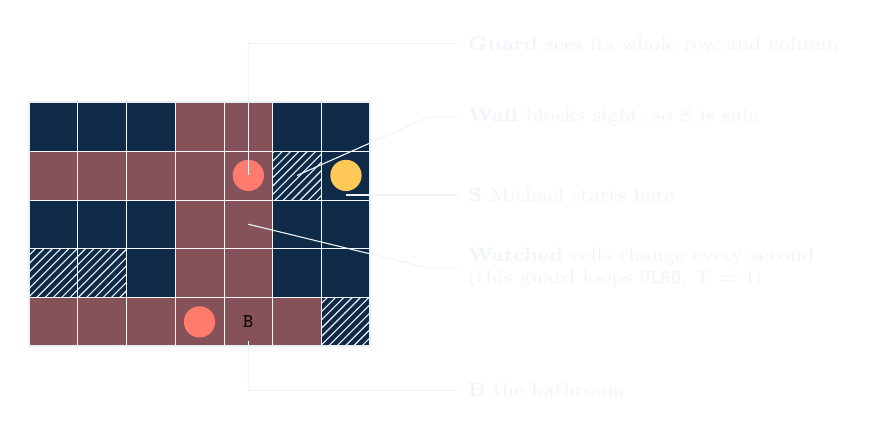
\begin{tikzpicture}[x=.62cm, y=.62cm]
    \plan{\Wzero}{\Gzero}{6/1}
    \begin{scope}[every node/.style={font=\scriptsize, align=left, anchor=west}]
      \draw[ink!70] (4.5,-1.5) -- (4.5,1.2) -- (8.8,1.2) node {\textbf{Guard} sees its whole row and column};
      \draw[ink!70] (5.5,-1.5) -- (8.2,-.3) -- (8.8,-.3) node {\textbf{Wall} blocks sight, so S is safe};
      \draw[ink!70] (6.5,-1.9) -- (8.2,-1.9) -- (8.8,-1.9) node {\textbf{S} Michael starts here};
      \draw[ink!70] (4.5,-2.5) -- (8.2,-3.4) -- (8.8,-3.4) node {\textbf{Watched} cells change every second\\(this guard loops \texttt{ULRD}, T = 4)};
      \draw[ink!70] (4.5,-4.9) -- (4.5,-5.9) -- (8.8,-5.9) node {\textbf{B} the bathroom};
    \end{scope}
  \end{tikzpicture}
  \vfill
  
\begin{tikzpicture}
    \node[box, font=\ttfamily\scriptsize, align=center, text width=13.2cm] {%
      each second: move or wait \quad\textperiodcentered\quad never stand in sight
      \quad\textperiodcentered\quad print fewest seconds to B, or CAUGHT
      \quad\textperiodcentered\quad R, C, T, G $\le$ 100};
  \end{tikzpicture}\par\smallskip
  {\ttfamily\tiny\color{amber}ESTIMATED DIFFICULTY: MEDIUM, KATTIS 3.5--4.5}
\end{frame}

% ================================================================ 3 filmstrip
\begin{frame}{Sample 1, step by step}
  \centering
  \renewcommand{\planfont}{\ttfamily\bfseries\tiny}
  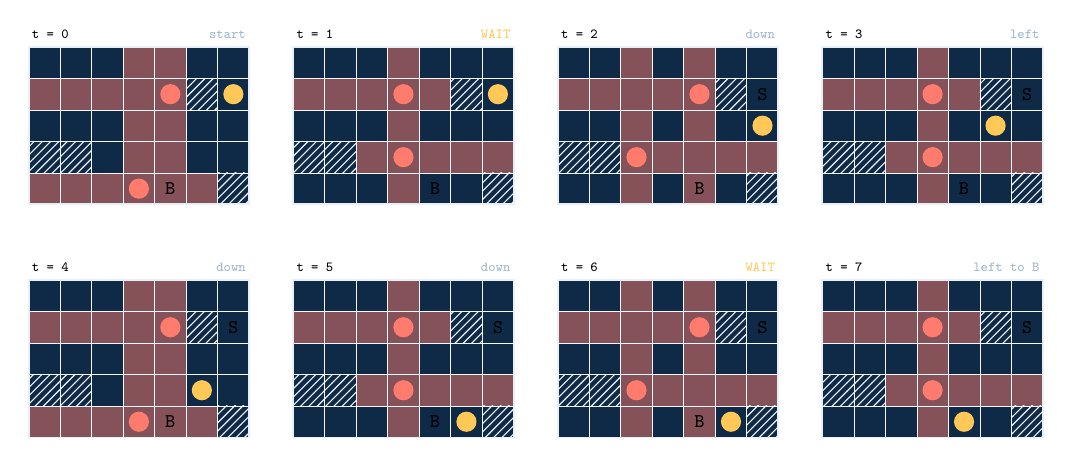
\begin{tikzpicture}[x=.4cm, y=.4cm]
    \foreach \t/\W/\G/\mc/\mr/\act/\col [count=\i from 0] in {
        0/\Wzero/\Gzero/6/1/start/dim, 1/\Wone/\Gone/6/1/WAIT/amber, 2/\Wtwo/\Gtwo/6/2/down/dim,
        3/\Wone/\Gone/5/2/left/dim, 4/\Wzero/\Gzero/5/3/down/dim, 5/\Wone/\Gone/5/4/down/dim,
        6/\Wtwo/\Gtwo/5/4/WAIT/amber, 7/\Wone/\Gone/4/4/left to B/dim} {
      \pgfmathsetmacro{\px}{mod(\i,4)*8.4}
      \pgfmathsetmacro{\py}{-int(\i/4)*7.4}
      \begin{scope}[shift={(\px,\py)}]
        \plan{\W}{\G}{\mc/\mr}
        \node[font=\ttfamily\tiny, anchor=south west, inner sep=1pt] at (0,.15) {t = \t};
        \node[font=\ttfamily\tiny\bfseries, anchor=south east, inner sep=1pt, text=\col] at (7,.15) {\act};
      \end{scope}
    }
  \end{tikzpicture}
  \vfill
  {\scriptsize\color{dim}Red: watched cells. Amber: Michael. The shortest path ignoring guards is 5 steps. Every route faster than 7 gets him seen.}
\end{frame}

% ================================================================ 4 insight
\begin{frame}{Key observation}
  \begin{columns}[c]
    \column{.42\textwidth}
      Every guard is home again after T seconds, so the restaurant at second $t$
      looks exactly like the restaurant at second $t \bmod T$.\par\bigskip
      {\ttfamily\color{amber}state = (cell, t mod T)}\par\medskip
      {\Large\bfseries $\le 100 \cdot 100 \cdot 100 = 10^6$}\\
      {\scriptsize\color{dim}states, so a plain BFS finishes in time}
    \column{.56\textwidth}\centering
      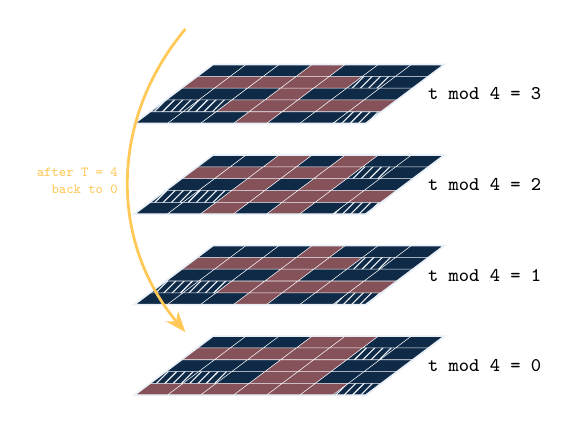
\begin{tikzpicture}
        \foreach \k/\W in {0/\Wzero, 1/\Wone, 2/\Wtwo, 3/\Wone} {
          \begin{scope}[shift={(0,\k*1.15)}, cm={.42,0,.2,.15,(0,0)}]
            \layer{\W}{t mod 4 = \k}
          \end{scope}
        }
        \draw[-{Stealth}, amber, line width=1pt] (-.35,3.9) to[bend right=40] node[left, font=\ttfamily\tiny, text=amber, align=right] {after T = 4\\back to 0} (-.35,.05);
      \end{tikzpicture}
  \end{columns}
\end{frame}

% ================================================================ 5 solution
\begin{frame}{Accepted solutions}
  \centering
  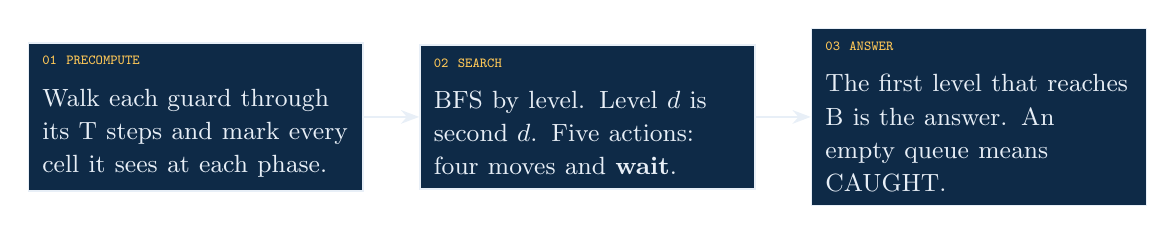
\begin{tikzpicture}[node distance=7mm, every node/.style={text width=3.9cm}]
    \node[box] (a) {{\ttfamily\tiny\color{amber}01 PRECOMPUTE}\\[1mm]
      \small Walk each guard through its T steps and mark every cell it sees at each phase.};
    \node[box, right=of a] (b) {{\ttfamily\tiny\color{amber}02 SEARCH}\\[1mm]
      \small BFS by level. Level $d$ is second $d$. Five actions: four moves and \textbf{wait}.};
    \node[box, right=of b] (c) {{\ttfamily\tiny\color{amber}03 ANSWER}\\[1mm]
      \small The first level that reaches B is the answer. An empty queue means CAUGHT.};
    \draw[-{Stealth}, ink, line width=.8pt] (a) -- (b);
    \draw[-{Stealth}, ink, line width=.8pt] (b) -- (c);
  \end{tikzpicture}
  \vfill
  \begin{columns}[t]
    \column{.45\textwidth}\centering
      {\ttfamily\tiny\color{dim}TIME}\\{\large\bfseries $O(RCT + GT(R+C))$}
    \column{.45\textwidth}\centering
      {\ttfamily\tiny\color{dim}MEMORY}\\{\large\bfseries $O(RCT)$}
  \end{columns}
  \vfill
\end{frame}

% ================================================================ 6 wrong answer
\begin{frame}{Wrong-answer solution}
  \centering
  
\begin{tikzpicture}
    \node[box, font=\ttfamily\small, text width=12.6cm] {%
      {\color{dim}accepted:}\ \ visited[\textcolor{amber}{t mod T}][r][c]\\
      {\color{dim}wrong:}\ \ \ \ \ seen[r][c]\hspace{1.2cm}{\color{alarm}\# never retried at a safer second}};
  \end{tikzpicture}\par\bigskip
  \begin{tikzpicture}[x=.34cm]
    \foreach \i in {0,...,38} {
      \pgfplotstablegetelem{\i}{wrong_ok}\of\bench
      \ifnum\pgfplotsretval=1
        \draw[ink!70, line width=.5pt] (\i+.08,0) rectangle (\i+.92,.84);
      \else
        \fill[amber] (\i+.08,0) rectangle (\i+.92,.84);
      \fi
    }
    \begin{scope}[decoration={brace, mirror, amplitude=3pt}, ink!70, every node/.style={tag, below=3pt, align=center}]
      \draw[decorate] (0,-.12) -- node {sample} (3,-.12);
      \draw[decorate] (3,-.12) -- node {secret01--10\\hand-made} (13,-.12);
      \draw[decorate] (13,-.12) -- node {secret11--29\\random} (32,-.12);
      \draw[decorate] (33,-.12) -- node {secret31--36\\timing traps} (39,-.12);
    \end{scope}
  \end{tikzpicture}\par\bigskip
  {\Large\bfseries\color{amber}10 of 39} {\small files fail, including Sample 1 and all six timing traps.}\\[1mm]
  {\scriptsize\color{dim}One square per test file, filled where the wrong-answer solution fails. Eight print CAUGHT when a safe route exists.}
\end{frame}

% ================================================================ 7 generator
\begin{frame}{Test-case generator}
  \begin{columns}[c]
    \column{.38\textwidth}
      {\Large\bfseries 14} {\small hand-made}\\
      {\scriptsize\color{dim}3 samples, 1$\times$2 grid, T = 1, single column, sealed-off B}\par\medskip
      {\Large\bfseries 19} {\small random}\\
      {\scriptsize\color{dim}seed 3212026: mazes, dense patrols, every limit at 100}\par\medskip
      {\Large\bfseries\color{amber}6} {\small timing traps}\\
      {\scriptsize\color{dim}seed 21993: kept only if the safe answer is longer than the shortest path ignoring guards}
    \column{.6\textwidth}
      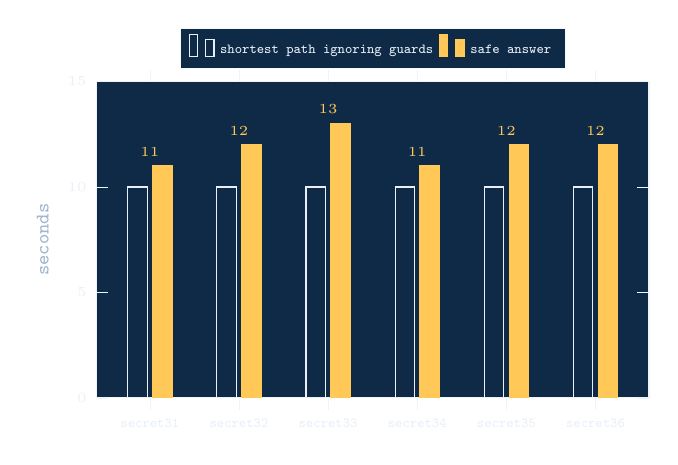
\begin{tikzpicture}
        \begin{axis}[blueprint, width=8.6cm, height=5.6cm, ybar, bar width=7pt,
            ymin=0, ymax=15, ytick={0,5,10,15},
            xtick={31,...,36}, xticklabels={secret31,secret32,secret33,secret34,secret35,secret36},
            x tick label style={font=\ttfamily\tiny}, enlarge x limits=.12,
            ylabel={seconds}, legend style={at={(.5,1.04)}, anchor=south}, legend columns=2]
          \addplot[draw=ink, fill=bp] coordinates {(31,10) (32,10) (33,10) (34,10) (35,10) (36,10)};
          \addplot[draw=amber, fill=amber, nodes near coords, every node near coord/.style={font=\ttfamily\tiny, text=amber}] coordinates {(31,11) (32,12) (33,13) (34,11) (35,12) (36,12)};
          \legend{shortest path ignoring guards, safe answer}
        \end{axis}
      \end{tikzpicture}
  \end{columns}
  \vfill
  {\scriptsize\color{dim}Every answer is rechecked, and 25 small cases are cross-checked against a second, independent solver.}
\end{frame}

% ================================================================ 8 test data
\begin{frame}{Test data}
  \begin{columns}[c]
    \column{.62\textwidth}
      \small\renewcommand{\arraystretch}{1.5}
      \begin{tabular}{@{}l >{\raggedright\arraybackslash}p{5.6cm}@{}}
        \textcolor{amber}{\ttfamily\scriptsize FILES} & \textcolor{amber}{\ttfamily\scriptsize WHAT THEY TEST} \\ \hline
        sample01--03 & The two examples from the statement, plus a wall detour \\
        secret01--10 & Hand-made edge cases: a 1$\times$2 grid, T = 1, one column, S and B walled apart \\
        secret11--29 & Random grids from 2$\times$2 up to 100$\times$100, with T and G up to 100 \\
        secret30 & A guard patrolling behind a wall \\
        secret31--36 & Timing traps, where Michael has to wait \\
      \end{tabular}
    \column{.36\textwidth}
      {\Large\bfseries 92,914} {\small bytes}\\
      {\scriptsize\color{dim}all inputs together, against a 50 MB limit}\par\medskip
      {\Large\bfseries 4,998} {\small seconds}\\
      {\scriptsize\color{dim}longest answer: a serpentine corridor (secret29)}\par\medskip
      {\Large\bfseries 19} {\small CAUGHT}\\
      {\scriptsize\color{dim}answers, including caught at t = 0 and a sealed-off B}\par\medskip
      {\scriptsize\color{dim}data/Description.txt explains every file.}
  \end{columns}
\end{frame}

% ================================================================ 9 validator
\begin{frame}{Input validator}
  \centering
  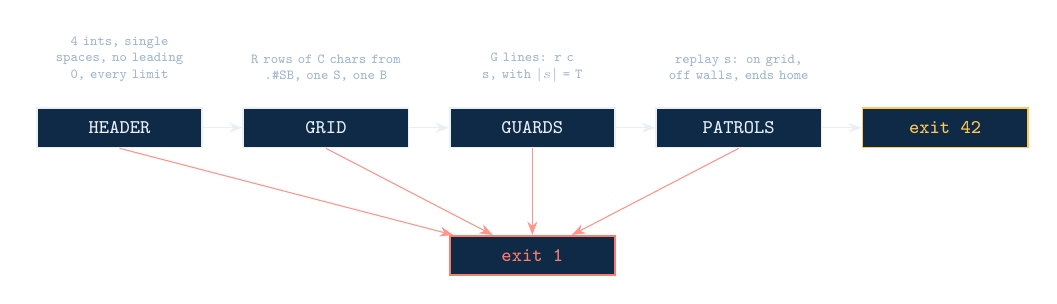
\begin{tikzpicture}[node distance=5mm, every node/.style={font=\ttfamily\scriptsize, minimum width=2.1cm, align=center}]
    \node[box] (h) {HEADER};
    \node[box, right=of h] (g) {GRID};
    \node[box, right=of g] (u) {GUARDS};
    \node[box, right=of u] (p) {PATROLS};
    \node[box, draw=amber, text=amber, right=of p] (ok) {exit 42};
    \foreach \a/\b in {h/g, g/u, u/p, p/ok} \draw[-{Stealth}, ink] (\a) -- (\b);
    \node[box, draw=alarm, text=alarm, below=11mm of u] (no) {exit 1};
    \foreach \a in {h,g,u,p} \draw[-{Stealth}, alarm!80, line width=.4pt] (\a.south) -- (no);
    \begin{scope}[every node/.style={tag, text width=2.1cm, minimum width=0pt, align=center, above=2mm}]
      \node at (h.north) {4 ints, single spaces, no leading 0, every limit};
      \node at (g.north) {R rows of C chars from .\#SB, one S, one B};
      \node at (u.north) {G lines: r c s, with $|s|$ = T};
      \node at (p.north) {replay s: on grid, off walls, ends home};
    \end{scope}
  \end{tikzpicture}\par\bigskip
  \begin{columns}[t]
    \column{.3\textwidth}\centering
      {\Large\bfseries 39 / 39}\\{\scriptsize\color{dim}real test files accepted}
    \column{.3\textwidth}\centering
      {\Large\bfseries\color{amber}0}\\{\scriptsize\color{dim}disagreements with a second parser on 3,000 mutated inputs}
    \column{.3\textwidth}\centering
      {\Large\bfseries 10 / 10}\\{\scriptsize\color{dim}broken inputs rejected, such as CRLF or an open patrol}
  \end{columns}
\end{frame}

% ================================================================ 10 experiments
\begin{frame}{Runtime experiments}
  \begin{columns}[c]
    \column{.66\textwidth}
      \begin{tikzpicture}
        \begin{axis}[blueprint, width=9.6cm, height=6.2cm, ymode=log, ymin=.01, ymax=2,
            xmin=0, xmax=40, xlabel={test file (sample01 \ldots{} secret36)}, ylabel={seconds},
            legend pos=north west, legend columns=3]
          \addplot[ink, mark=*, mark size=1.2pt] table[x=idx, y=python] {\bench};
          \addplot[amber, mark=*, mark size=1.2pt] table[x=idx, y=java] {\bench};
          \addplot[alarm, dashed, mark=none] table[x=idx, y=wrong] {\bench};
          \legend{Python, Java, wrong answer}
        \end{axis}
      \end{tikzpicture}
    \column{.32\textwidth}
      {\ttfamily\tiny\color{dim}WORST FILE: secret21, 100$\times$100, T = 100}\par\smallskip
      {\Large\bfseries 1.01 s} {\small Python}\\
      {\Large\bfseries\color{amber}0.053 s} {\small Java}\par\medskip
      {\ttfamily\tiny\color{dim}ALL 39 FILES}\par\smallskip
      {\small 2.30 s Python \textperiodcentered{} 1.29 s Java}\par\medskip
      {\scriptsize\color{dim}Most of Java's per-file time is JVM start-up. Both accepted solutions pass all 39 files. The wrong answer is even faster and still fails 10.}
  \end{columns}
  \vfill
  {\ttfamily\tiny\color{dim}median of 3 runs per file, start-up included, on a laptop}
\end{frame}

% ================================================================ 11 debrief
\begin{frame}{Reflection}
  \centering
  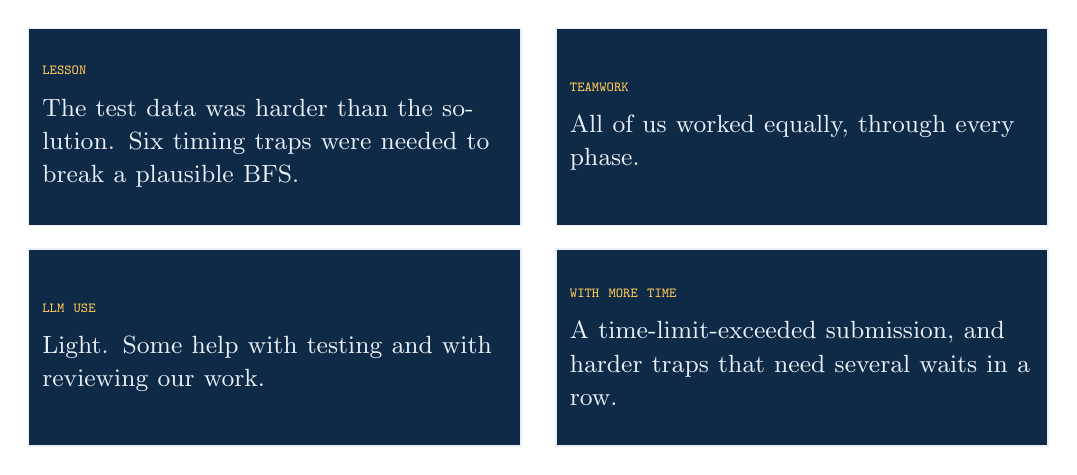
\begin{tikzpicture}[every node/.style={box, text width=5.9cm, minimum height=2.5cm, anchor=north west}]
    \node at (0,0) {{\ttfamily\tiny\color{amber}LESSON}\\[1mm]\small
      The test data was harder than the solution. Six timing traps were needed to break a plausible BFS.};
    \node at (6.7,0) {{\ttfamily\tiny\color{amber}TEAMWORK}\\[1mm]\small
      All of us worked equally, through every phase.};
    \node at (0,-2.8) {{\ttfamily\tiny\color{amber}LLM USE}\\[1mm]\small
      Light. Some help with testing and with reviewing our work.};
    \node at (6.7,-2.8) {{\ttfamily\tiny\color{amber}WITH MORE TIME}\\[1mm]\small
      A time-limit-exceeded submission, and harder traps that need several waits in a row.};
  \end{tikzpicture}
\end{frame}

\end{document}
